\cleardoublepage
\chapter{Introduction}
\label{sec:intro}
\pagenumbering{arabic} % para empezar la numeración de página con números

\section{General context}

An Unmanned Aerial Vehicle (UAV) is an aircraft able to fly without any pilot or operator on board. They may be operated through remote control by a human operator or with various degrees of autonomy, from sensor-driven control aids provided to the operator to fully autonomous flight through preplanned missions.
UAVs have existed since the 20th century and were initially developed as military technology to protect pilots from dangerous missions.
However, as the cost of the electronics and sensors decreased and control technologies improved, they became available to a broader public. They are now employed in various civil applications like crop control, search and rescue, or filmmaking and photography.
Nevertheless, most commercial solutions are limited to remote operations or rudimentary autonomy, with fully autonomous flight still in the earliest phases.
However, there is a growing trend towards using vision-based control solutions, which can offer improved performance and flexibility compared to traditional control methods.
Vision-based control solutions use cameras and image processing algorithms to provide real-time feedback and control of the UAV. 
These solutions are often more flexible and robust than traditional control methods, which are typically based on accelerometers, gyroscopes, and other sensors. 
Additionally, vision-based control solutions can be implemented on low-cost platforms, making them accessible to a broader range of users.
These vision-based guidance systems have only started to appear in recent years as artificial intelligence becomes more widespread and very few fully-developed consumer-ready platforms are available for the general public.
Even so,
from the essential hardware to build an own quadcopter, a helicopter with four rotors that represents the most common type of UAV, to miniaturized computers that handle complex calculations and open-source software that can be customized to endless applications,
all the individual pieces that enable building such a system are readily available.

\section{The Dronecontrol project}

The project presented in this thesis aims to show the options available to design and implement control solutions for the popular PX4 open-source autopilot platform and how to integrate them with detection and tracking computer vision mechanisms to achieve simple vision-based self-guided UAVs.
All the necessary code for this project has been written in Python and always runs outside the flight controller board on a companion computer.
This allows more processing power to be accessible for any compute-intensive computer vision algorithms,
but also ensures that the control solutions are abstracted from the hardware components and not dependent on the specific flight stack employed, 
to allow applying the results to any available autopilot platform with exposed APIs.
Two complete vision-based control solutions have been implemented for two scenarios: keeping the machine driving the computer vision algorithms onboard or offboard the vehicle during flight.
The following chapters detail the hardware, libraries, testing environments, and systems used during the development process and how they can be used to develop new control solutions based on available computer vision mechanisms.

\section{Objectives}
\label{sec:objetives}

The main objective of this project is to demonstrate the available possibilities to develop control solutions for the PX4 autopilot driven by computer vision mechanisms.

More specifically, it aims to:
\begin{itemize}
    \item Introduce the software and hardware environment of the Dronecode project and the techniques they have made available.
    \item Show the minimum requirements needed to develop control software for the platform.
    \item Suggest viable vision-driven control solutions that use those techniques.
    \item Present a testing process using available tools that can help ensure safety and reliability for any new solutions developed.
    \item Build a quadcopter and use it to carry out test flights with the developed solutions.
\end{itemize}


\section{Time planning}
\label{sec:time-planning}

\begin{figure}
  \centering
  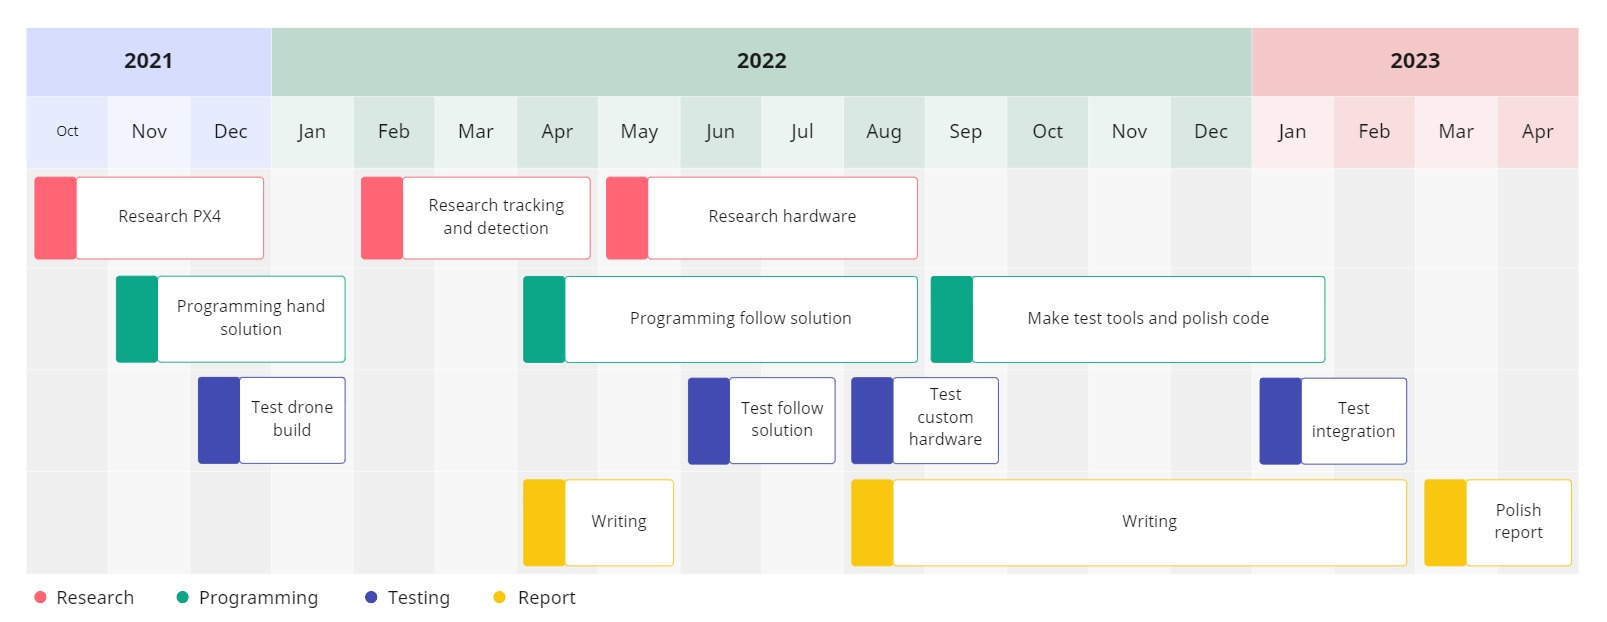
\includegraphics[width=\textwidth,keepaspectratio]{img/project-timeline.jpg}
  \caption{Timeline for the development of the project}
  \label{fig:project-timeline}
\end{figure}

This project has been carried out over a natural period of one and a half years due to having to coordinate with working a full-time job in parallel.
The development has been spread out over three phases, taking up a total of 400 hours of dedication to the project.
Each of these phases can be divided into three main tasks: research of the necessary systems, programming of custom solutions and tools, and comprehensive testing on different scenarios.
Additionally, during the last two phases, time was allocated to the process of writing the report, which occurred concurrently with the research and development work.


\begin{itemize}
    \item Phase 1: Proof-of-concept ( Oct 21 - Jan 22: 61 hours )
    \begin{itemize}
        \item Research PX4 (12 hours)
        \item Programming hand solution (42 hours)
        \item Test standard drone build (7 hours)
    \end{itemize}
    \item Phase 2: Follow solution ( Feb 22 - Aug 22: 138 hours )
    \begin{itemize}
        \item Research tracking and detection (33 hours)
        \item Programming follow solution (80 hours)
        \item Test custom hardware (25 hours)
    \end{itemize}
    \item Phase 3: Hardware ( Sep 22 - Feb 23: 65 hours )
    \begin{itemize}
        \item Research hardware (15 hours)
        \item Make test tools and polish code (33 hours)
        \item Test custom hardware and integration (17 hours)
    \end{itemize}
    \item Writing report (133 hours)
\end{itemize}


\section{Thesis layout}
\label{sec:layout}

This section details the structure of this thesis.
It is organized into five chapters that reflect the three distinct tasks described in the last section: research, development and testing, along with this introduction and some final conclusions.
Specifically:

\begin{itemize}
    \item In the first chapter, there is a brief introduction to the context in which the project has been developed, as well as the objectives it pursues.
    \item Chapter 2 presents the technologies and tools employed in this project and the current state-of-the-art for UAV vision-based control solutions.
    \item The third chapter introduces the simulation environments used to develop the solutions throughout the project and the architecture of the hardware and software used.
    \item Chapter 4 follows along through the process of testing every part of the system incrementally until reaching the final flight tests.
    \item The last chapter shows the conclusions drawn from the work and presents ideas for future development.
\end{itemize}


\cleardoublepage